\documentclass{beamer}


%%%%%%%%%%%%%%%%%%%%%%%%%%%%%%%%%%%%%%%%%%%%%%%%%%%%%%%%%%%%%%%%%%%%%%%%%%%%%%
% Definición del formato/estilo de Beamer 
%%%%%%%%%%%%%%%%%%%%%%%%%%%%%%%%%%%%%%%%%%%%%%%%%%%%%%%%%%%%%%%%%%%%%%%%%%%%%%
\usetheme{Warsaw}
%\usetheme{Darmstadt} 
%\usetheme{Frankfurt} 
%\usetheme{Goettingen}
%\usetheme{Dresden}
%\usetheme{Madrid}
%\usetheme{Marburg}
%\usetheme{Montpellier}
%\usetheme{Rochester} 
%\usetheme{Singapore}
%\usetheme{Szeged}
%\usecolortheme{albatross}
%\usecolortheme{seahorse}  
%\usecolortheme{beetle}
%\usecolortheme{crane}
%\usecolortheme{dolphin}
%\usecolortheme{dove}
%\usecolortheme{fly}
%\usecolortheme{lily}
%\usecolortheme{orchid}
%\usecolortheme{rose}
%\usecolortheme{seagull}
%\usecolortheme{whale}
\usefonttheme{professionalfonts}

\definecolor{pantone254}{RGB}{122,59,122}
\definecolor{pantone3015}{RGB}{0,88,147}
\definecolor{pantone432}{RGB}{56,61,66}
\setbeamercolor*{palette primary}{use=structure,fg=white,bg=pantone254}
\setbeamercolor*{palette secondary}{use=structure,fg=white,bg=pantone3015}
\setbeamercolor*{palette tertiary}{use=structure,fg=white,bg=pantone432}
\setbeamercolor*{palette sidebar primary}{use=structure,fg=pantone254}
\setbeamercolor*{palette sidebar tertiary}{use=structure,fg=pantone3015}
\setbeamercolor*{block title}{bg=pantone432,fg=white}
\setbeamercolor*{alerted text}{fg=pantone254}
\setbeamercolor*{item projected}{fg=pantone254}
\setbeamercolor*{section in toc shaded}{use=structure,fg=structure.fg}
\setbeamercolor*{section in toc}{fg=pantone3015}
\setbeamercolor*{subsection in toc shaded}{fg=pantone3015}
\setbeamercolor*{subsection in toc}{fg=pantone432}


%%%%%%%%%%%%%%%%%%%%%%%%%%%%%%%%%%%%%%%%%%%%%%%%%%%%%%%%%%%%%%%%%%%%%%%%%%%%%%
% Paquetes auxiliares
%%%%%%%%%%%%%%%%%%%%%%%%%%%%%%%%%%%%%%%%%%%%%%%%%%%%%%%%%%%%%%%%%%%%%%%%%%%%%%
\usepackage[utf8]{inputenc}
\usepackage[spanish]{babel}
\usepackage{algorithm}
\usepackage{algorithmic}
\usepackage{latexsym,amsbsy,amssymb,amsfonts,amsmath,bbm}
\usepackage{dsfont}
\usepackage{color}
\usepackage{multirow}
\usepackage{fancybox}
\usepackage{fancyvrb}
\usepackage{verbatim}
\usepackage{verbatimbox}
\usepackage{graphicx}
\usepackage[export]{adjustbox}
\usepackage{minted}
\usepackage{hyperref}


%%%%%%%%%%%%%%%%%%%%%%%%%%%%%%%%%%%%%%%%%%%%%%%%%%%%%%%%%%%%%%%%%%%%%%%%%%%%%%
% Definición de comandos 
%%%%%%%%%%%%%%%%%%%%%%%%%%%%%%%%%%%%%%%%%%%%%%%%%%%%%%%%%%%%%%%%%%%%%%%%%%%%%%
\newcommand{\PC}{\mbox{\textsc{pc}}}


%%%%%%%%%%%%%%%%%%%%%%%%%%%%%%%%%%%%%%%%%%%%%%%%%%%%%%%%%%%%%%%%%%%%%%%%%%%%%%
% Formato
%%%%%%%%%%%%%%%%%%%%%%%%%%%%%%%%%%%%%%%%%%%%%%%%%%%%%%%%%%%%%%%%%%%%%%%%%%%%%%
%\newcommand*\oldmacro{}
%\let\oldmacro\insertshortauthor% save previous definition
%\renewcommand*\insertshortauthor{%
%\leftskip=.3cm% before the author could be a plus1fill ...
%\insertframenumber\,/\,\inserttotalframenumber\hfill\oldmacro}

%\usebackgroundtemplate{\includegraphics[width=0.5\paperheight]{images/fondoULL}}
%\logo{\includegraphics[width=0.1\paperheight]{images/logoULL}}
\setbeamersize{text margin left=.5cm,text margin right=.5cm}


%%%%%%%%%%%%%%%%%%%%%%%%%%%%%%%%%%%%%%%%%%%%%%%%%%%%%%%%%%%%%%%%%%%%%%%%%%%%%%%%
\begin{document}

% Formato
%\setbeamertemplate{footline}[page number]
%\setbeamertemplate{navigation symbols}{}

\title{Trabajo Fin de Máster}
\author{Carlos Díaz Calzadilla}

\date{Curso 2022-2023}


%-------------------------------------------------------------------------------
% Portada
%-------------------------------------------------------------------------------
\newcommand{\HRule}{\rule{\linewidth}{0.75mm}}

\begin{frame}
\begin{center}
\thispagestyle{empty}

	%\vspace{-2cm}
	
\includegraphics[width=0.5\textwidth]{Presentacion/escuela-doctorado-posgrado-original.png}\\
	%\vspace{0.5cm}
	\textsc{\Large Trabajo Fin de Máster}\\
	\vspace{0.25cm}
	\textsc{\Large Escuela de Doctorado y Posgrado}\\
	%\HRule \\[0.35cm]
	\vspace{0.5cm}
	\begin{huge}
	%\shadowbox{{{\Large \bfseries Tema 0: Conceptos Básicos}}}\\[0.25cm]
	\begin{alertblock}{}
		\vspace{0.4cm}
		\center{Generador estático web para facilitar tareas en la docencia}
		\vspace{0.4cm}
	\end{alertblock}
	\end{huge}
	\textsc{Autor: Carlos Díaz Calzadilla}\\
	\textsc{Tutor: Casiano Rodríguez León}\\
	%{\bfseries Conceptos Básicos}\\[0.2cm]
	\vspace{0.5cm}
	%\HRule \\[0.7cm]
	\footnotesize{Curso 2022-2023}
\end{center}
\end{frame}


%-------------------------------------------------------------------------------
% Tabla de contenidos
\begin{frame}[allowframebreaks]
\frametitle{Indice}
\tableofcontents
\end{frame} 

        \begin{frame}{Indice}
            \begin{enumerate}
                \item Introducción
                \item Tecnologías utilizadas
                \item Diseño del sistema
                \item Implementación
                \item Conclusiones y líneas futuras
                \item Bibliografía
            \end{enumerate}
        \end{frame}


        \begin{frame}{Introducción - Antecedentes y estado actual del arte}
            \begin{center}
            	
\includegraphics[width=.55\textwidth]{Presentacion/introduccion/lms.png} 
            	
\includegraphics[width=.35\textwidth]{Presentacion/introduccion/git.png}    
            \end{center}
        \end{frame}

        \begin{frame}{Introducción - GitHub Education}
            \begin{center}
            	
\includegraphics[width=.55\textwidth]{Presentacion/introduccion/githubedu.png}
                \begin{itemize}
                    \item Plataforma de presentación:
                    \begin{itemize}
                        \item Repositorio público (base)
                        \item Repositorio privado (por estudiante)
                    \end{itemize}
                    \item Alojamiento del material del curso
                \end{itemize}
            \end{center} 
            
        \end{frame}

        \begin{frame}{Introducción - Objetivos}
            \begin{enumerate}
                \item Autorización de usuario ocultando contenido dependiendo de rol asignado.
                \item Conectar aplicación con GitHub (facilitar roles) y obtener información mediante su API.
                \item Despliegue sencillo y añadir guía de uso.
                \item Crear script para facilitar tareas de creación de entorno y configuración inicial.
            \end{enumerate}            
        \end{frame}
    	

        \begin{frame}{Tecnologías utilizadas - Bash}
        
    		\begin{center}
                
\includegraphics[width=1\textwidth]{Presentacion/tecnologias/home.png}\hfill
    		\end{center}  
            
        \end{frame}

        \begin{frame}{Tecnologías utilizadas - Vue}
        
    		\begin{figure}[htp]
                \centering
                
\includegraphics[width=1\textwidth]{Presentacion/tecnologias/vuejs.png}\hfill
                \label{fig:vuejs}
    		\end{figure}  
            
        \end{frame}

        \begin{frame}{Tecnologías utilizadas - Vue}
        
    		\begin{figure}[htp]
                \centering
                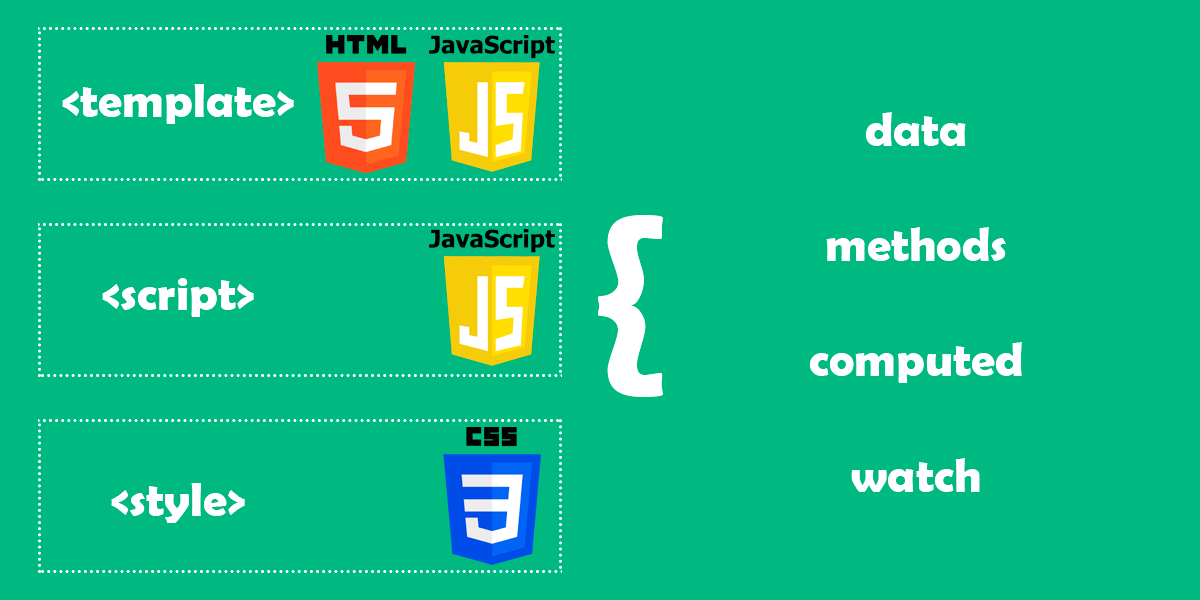
\includegraphics[width=1\textwidth]{Presentacion/tecnologias/sfc.png}\hfill
                \label{fig:sfc}
                \caption{Estructura componentes}
    		\end{figure}  
            
        \end{frame}

        \begin{frame}{Tecnologías utilizadas - Vuex}
        
    		\begin{center}
                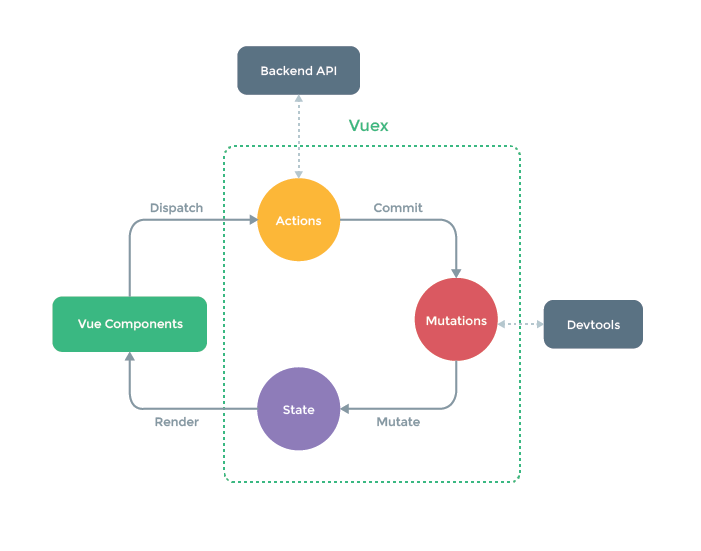
\includegraphics[width=.8\textwidth]{Presentacion/tecnologias/vuex.png}\hfill
    		\end{center}  
            
        \end{frame}

        \begin{frame}{Tecnologías utilizadas - Generador de sitios estáticos}
        
    		\begin{center}
                
\includegraphics[width=.8\textwidth]{Presentacion/tecnologias/ssg.png}\hfill
    		\end{center}  

            \begin{table}[!h]
                \centering
                \begin{tabular}{c|c}
                     Ventajas & Desventajas \\ \hline
                     Alta velocidad & Contenido a tiempo real \\
                     Seguridad & Interacción del usuario \\
                     Mantenimiento & \\
                \end{tabular}
                \caption{Ventajas frente a desventajas}
                \label{tab:ventajas}
            \end{table}
            
        \end{frame}

        \begin{frame}{Tecnologías utilizadas - Generador de sitios estáticos}

            \begin{center}
                
\includegraphics[width=.45\textwidth]{Presentacion/tecnologias/vitepress.png}
                
\includegraphics[width=.45\textwidth]{Presentacion/tecnologias/vuepress.png}   
            \end{center}
            
        \end{frame}

        \begin{frame}{Tecnologías utilizadas - Firebase}
        
            \begin{center}
                \begin{figure}[htp]
                    \centering
                    
\includegraphics[width=.7\textwidth]{Presentacion/tecnologias/firebase.png}\hfill
                    \label{fig:fir}
                \end{figure}  
    
                \begin{itemize}
                    \item Autenticación a través de diferentes proveedores
                    \item Hosting
                \end{itemize}
            \end{center}            
            
        \end{frame}
     
    \begin{frame}{Diseño del sistema}

            \begin{center}
                \begin{table}[]
                    \begin{tabular}{c|c}
                         Cliente-servidor & Local \\ \hline
                         & \\
                         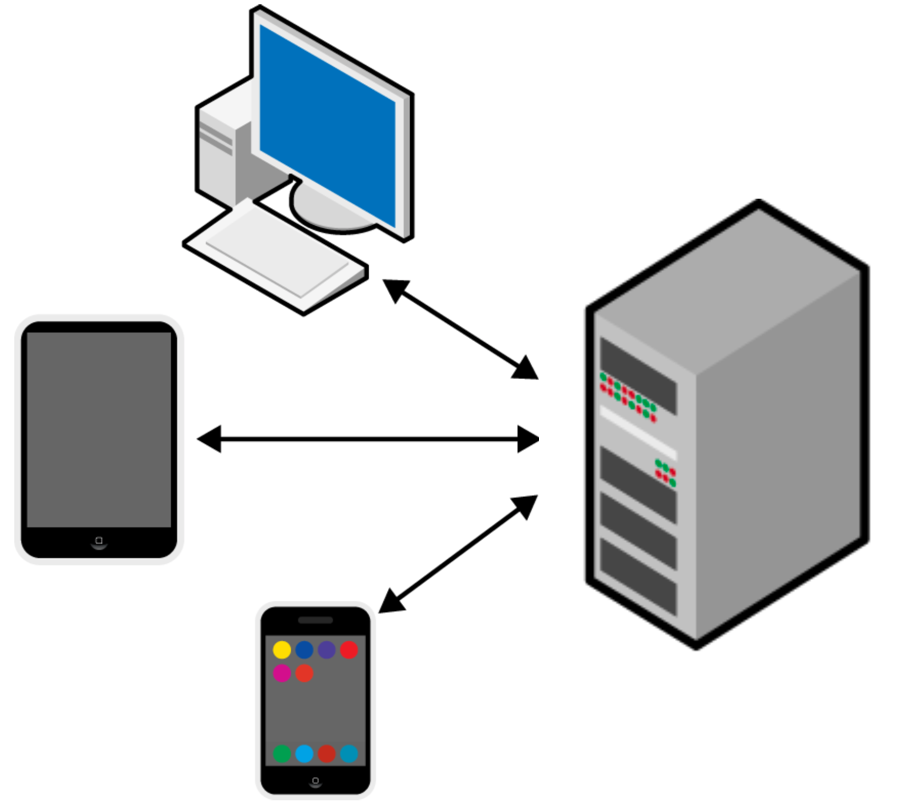
\includegraphics[width=.5\textwidth]{Presentacion/diseño/client-server.png} & 
\includegraphics[width=.25\textwidth]{Presentacion/diseño/client.png} \\
                    \end{tabular}
                \end{table}
                   
            \end{center}
        
    \end{frame}   

    \begin{frame}{Diseño del sistema - Script}
    
        \begin{enumerate}
            \item Clonar repositorio
            \item Definir la configuración inicial
            \item Autenticación a través de Firebase
            \item Configuración firebase
            \item Construcción y despliegue del sitio
        \end{enumerate}
        
    \end{frame}  

    \begin{frame}{Diseño del sistema - Plantilla}

        \begin{figure}
            \centering
            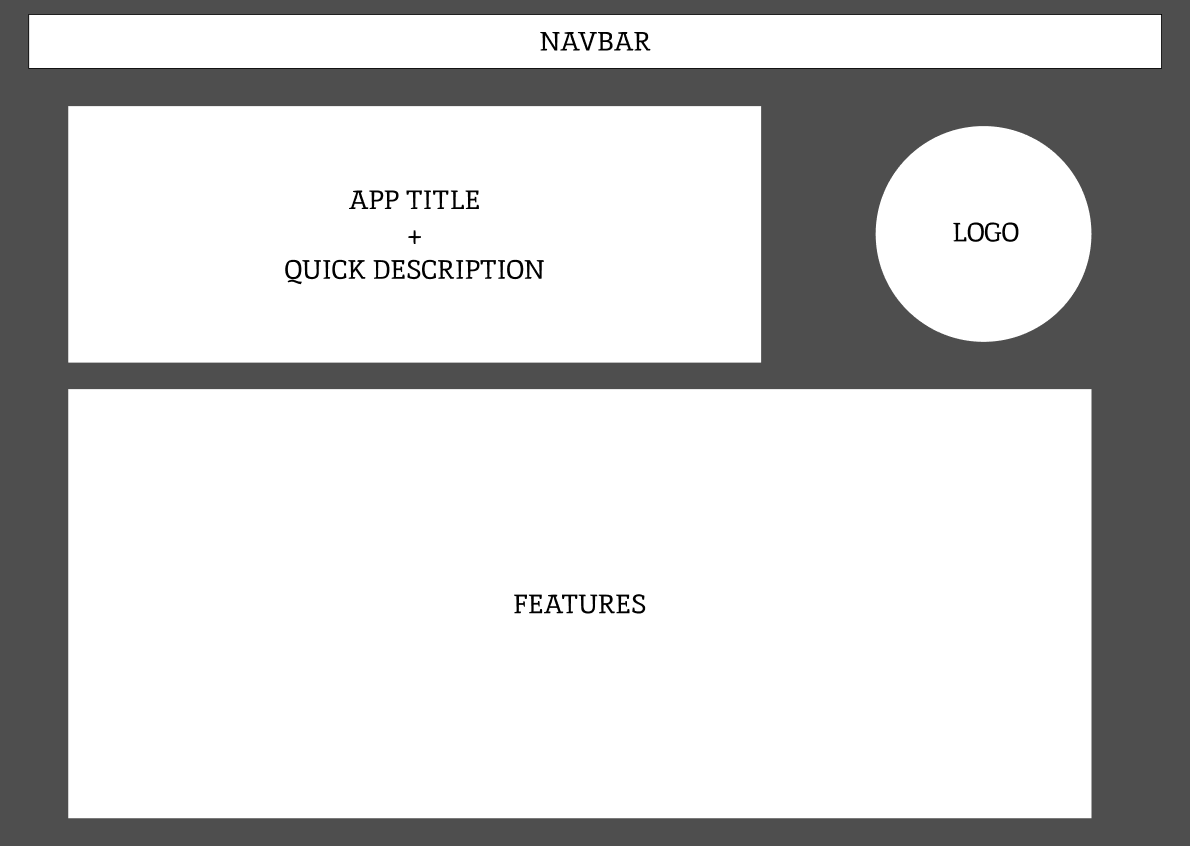
\includegraphics[width=.8\textwidth]{Presentacion/mockup/initial.png}
            \caption{Diseño inicial página principal}
        \end{figure}
        
    \end{frame}  

    \begin{frame}{Diseño del sistema - Plantilla}

        \begin{figure}
            \centering
            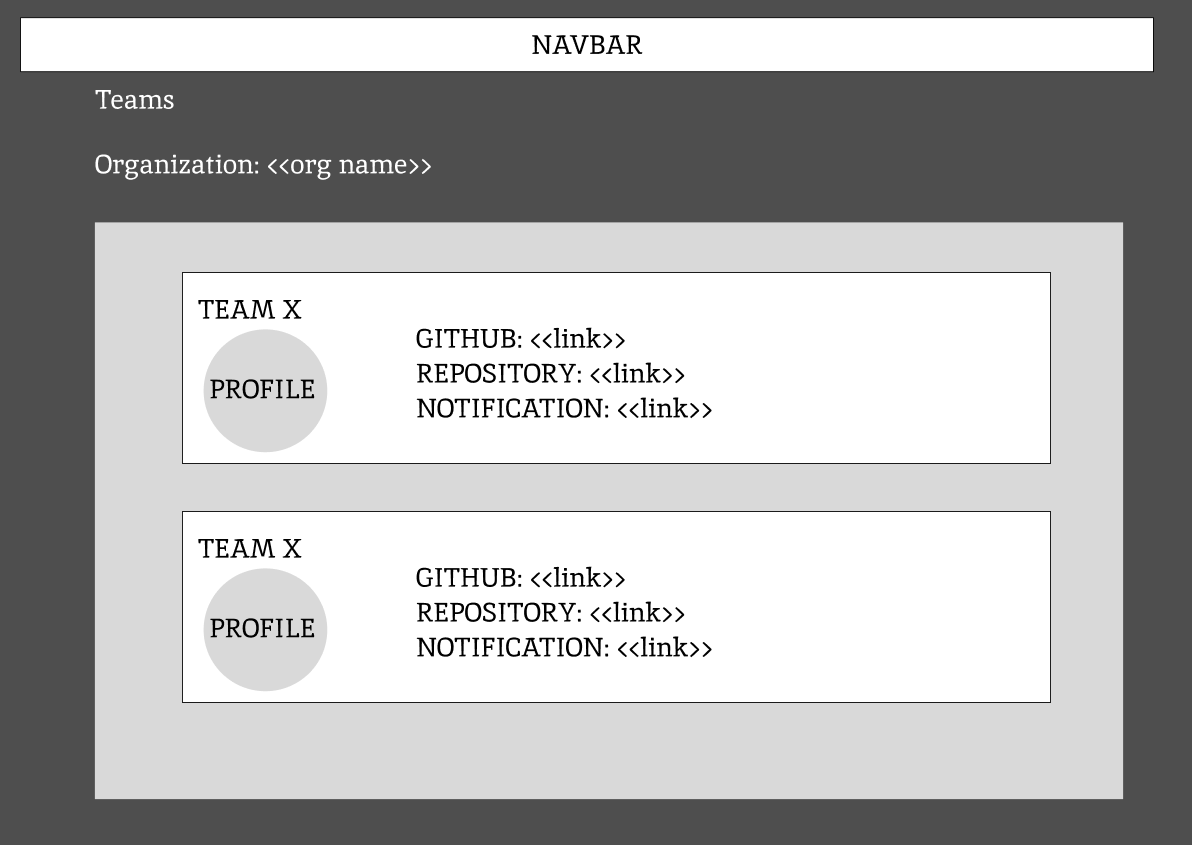
\includegraphics[width=.8\textwidth]{Presentacion/mockup/teams.png}
            \caption{Diseño inicial teams}
        \end{figure}
        
    \end{frame}  

    \begin{frame}{Diseño del sistema - Plantilla}

        \begin{figure}
            \centering
            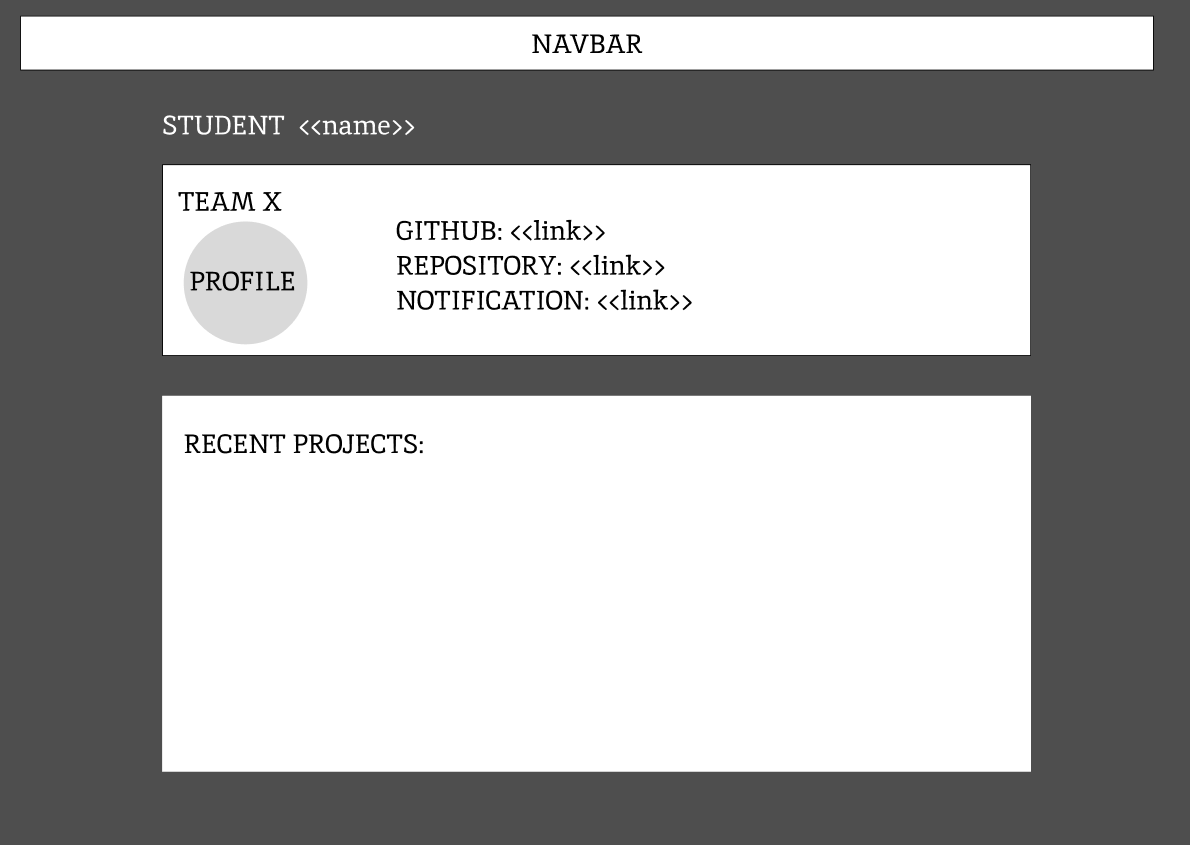
\includegraphics[width=.8\textwidth]{Presentacion/mockup/student.png}
            \caption{Diseño inicial team}
        \end{figure}
        
    \end{frame}  

    \begin{frame}{Diseño del sistema - Plantilla}

        \begin{figure}
            \centering
            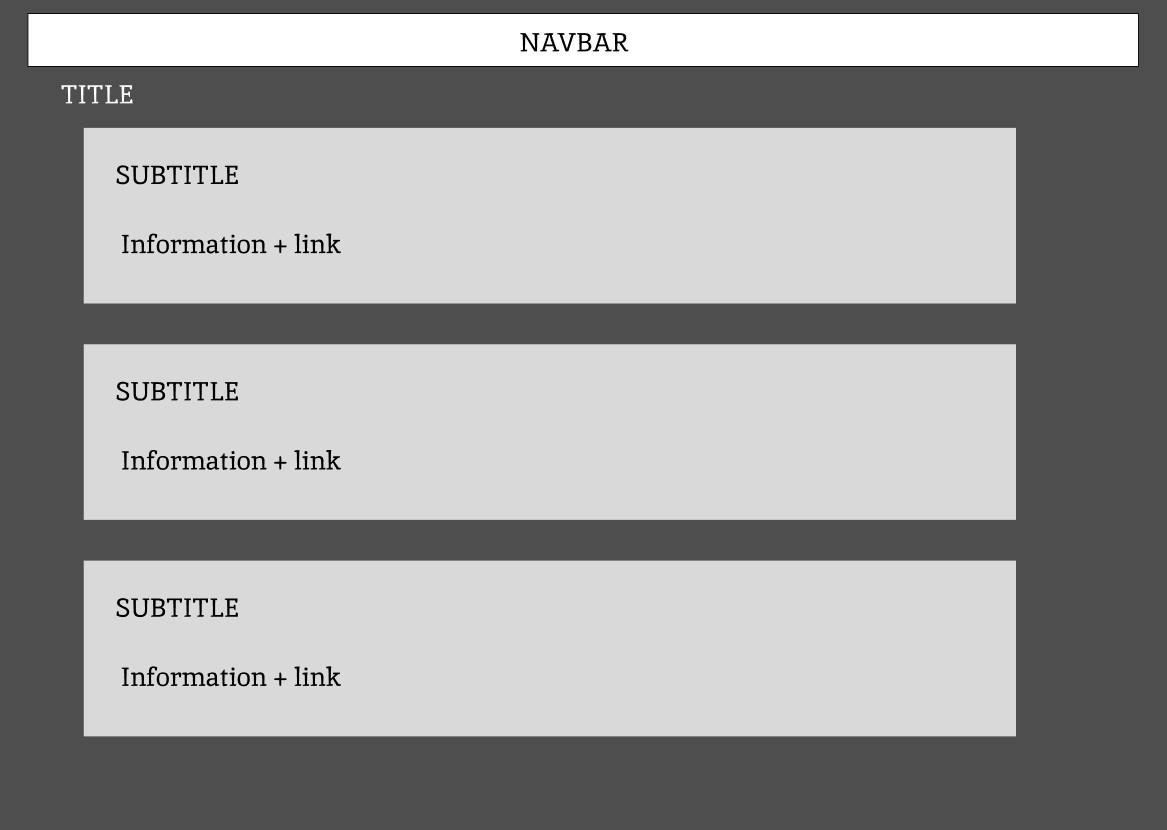
\includegraphics[width=.8\textwidth]{Presentacion/mockup/other.png}
            \caption{Diseño inicial para tareas, unidades y lecciones}
        \end{figure}
        
    \end{frame}  

    \begin{frame}{Diseño del sistema - Plantilla}

        \begin{figure}
            \centering
            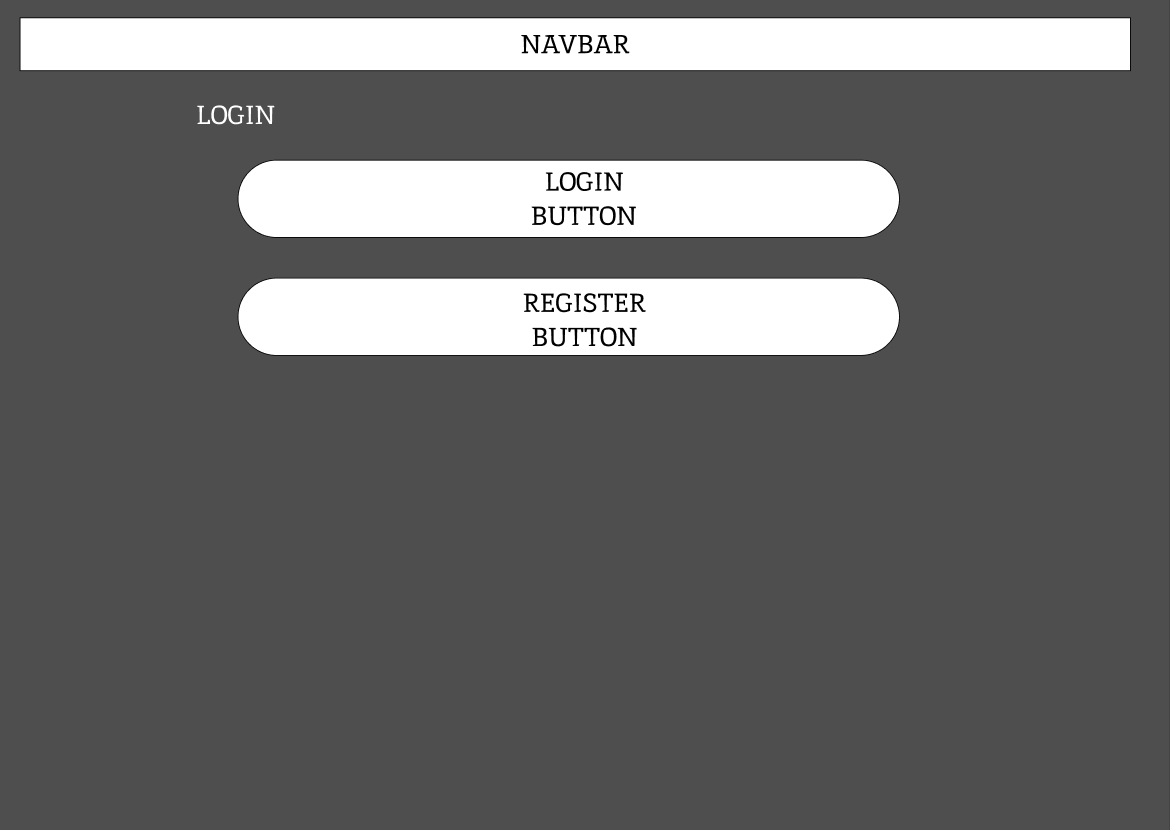
\includegraphics[width=.8\textwidth]{Presentacion/mockup/general login.png}
            \caption{Diseño inicial vista autenticación}
        \end{figure}
        
    \end{frame}  

    \begin{frame}{Diseño del sistema - Plantilla}

        \begin{figure}
            \centering
            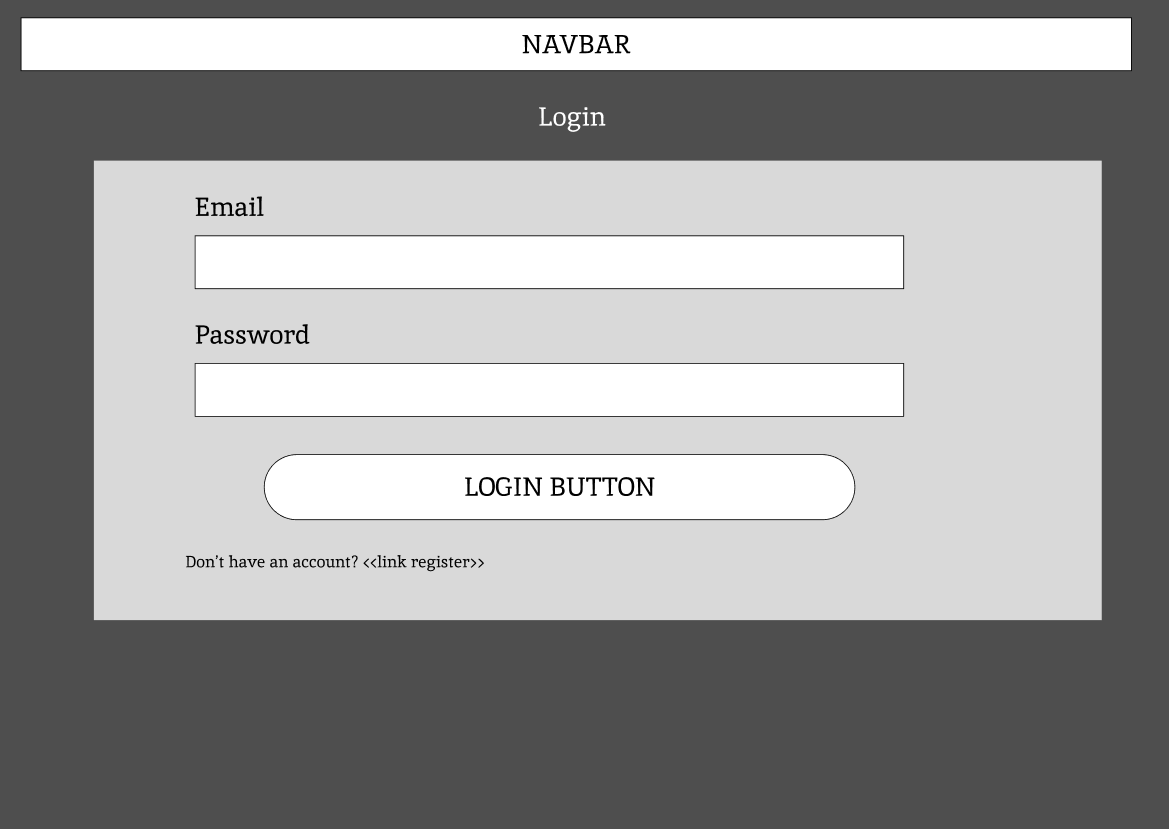
\includegraphics[width=.8\textwidth]{Presentacion/mockup/login.png}
            \caption{Diseño inicial acceso}
        \end{figure}
        
    \end{frame}  

    \begin{frame}{Diseño del sistema - Plantilla}

        \begin{figure}
            \centering
            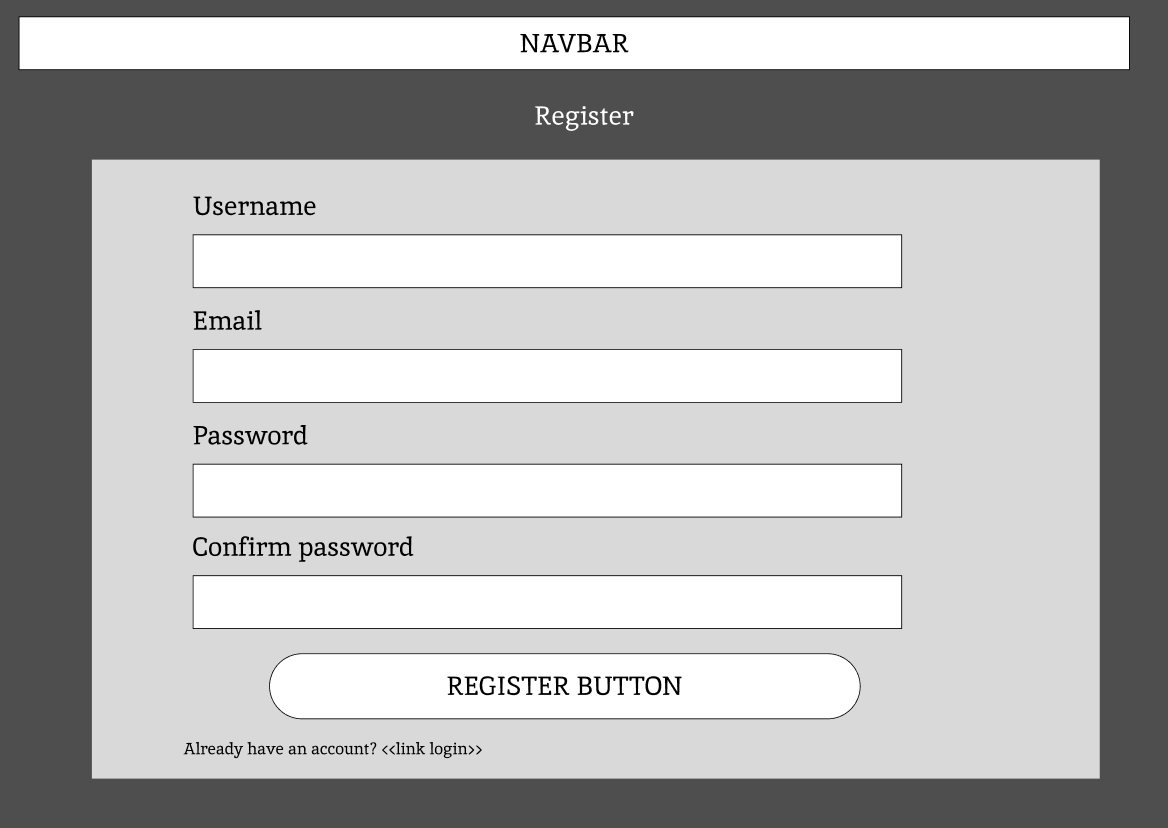
\includegraphics[width=.8\textwidth]{Presentacion/mockup/register.png}
            \caption{Diseño inicial registro}
        \end{figure}
        
    \end{frame}  

    \begin{frame}{Implementación - Script}

        \begin{block}{Estructura script}
            Es importante conocer la estructura, tanto del script como de la plantilla, para entender como ha sido implementado
            
        \end{block}

        \begin{center} 
            \begin{figure}
                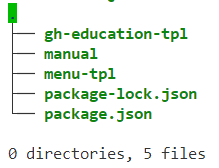
\includegraphics[width=.45\textwidth]{Presentacion/implementacion/script-structure.png}
                \caption{Estructura Script}
            \end{figure}
        \end{center}
        
        
    \end{frame}  

    \begin{frame}{Implementación - Script}
    
        \begin{block}{Manual script}
            Para poder realizar una documentación de los archivos implementados en bash, se pueden crear manuales que luego se acceden utilizando la sintaxis: {\tt man <paquete>}
            
        \end{block}

        \begin{center}  
            \begin{figure}
                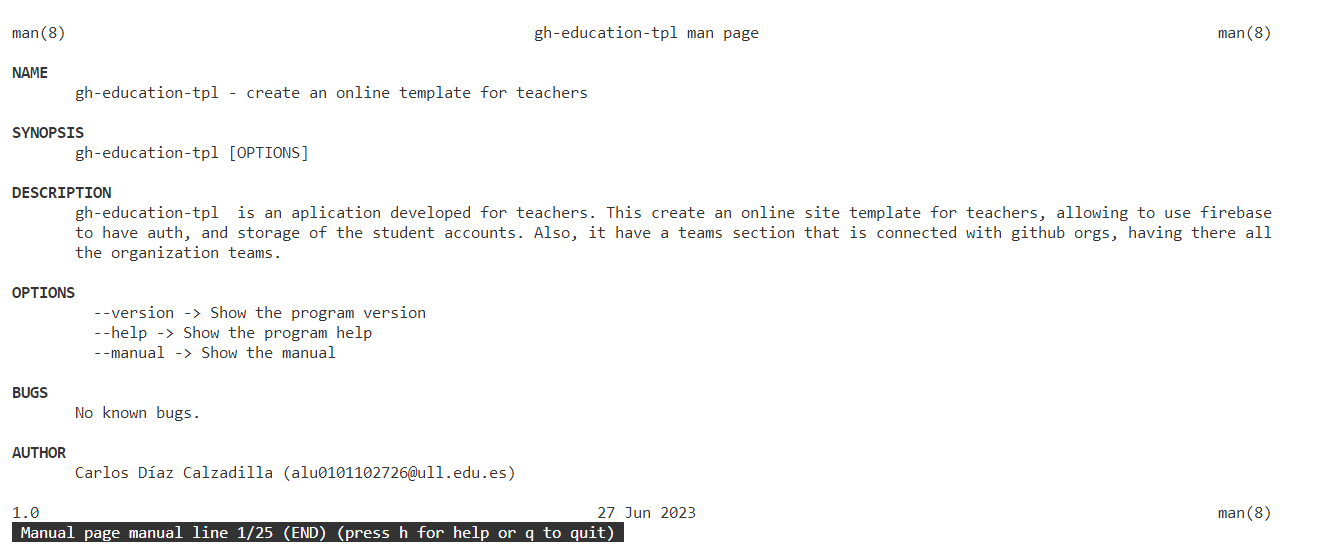
\includegraphics[width=.9\textwidth]{Presentacion/implementacion/script/manual.png}
                \caption{Manual Script}
            \end{figure}            
        \end{center}
        
        
    \end{frame}  

    \begin{frame}{Implementación - Script}
    
        \begin{block}{Menu script}
            Con el objetivo de que la navegación por parte del usuario fuera más cómoda y sencilla a la hora de moverse para seleccionar las opciones, este script, se encarga de gestionar dichos movimientos (que se realizan presionando las flechas del teclado) y de la opción seleccionada.
            
        \end{block}

        \begin{center}  
            \begin{figure}
                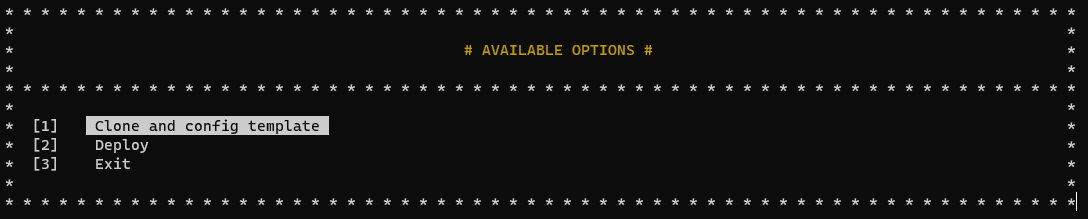
\includegraphics[width=.9\textwidth]{Presentacion/implementacion/script/home.png}
                \caption{Ejemplo menu en el script}
            \end{figure}            
        \end{center}
        
        
    \end{frame}  

    \begin{frame}{Implementación - Script}
    
        \begin{block}{Script principal}
            Por último, el script principal, va a permitir al usuario configurar, trabajar e incluso desplegar el sitio, el menú inicial es variable dependiendo si ya se ha clonado la plantilla o si no.            
        \end{block}

        \begin{center}  
            \begin{figure}
                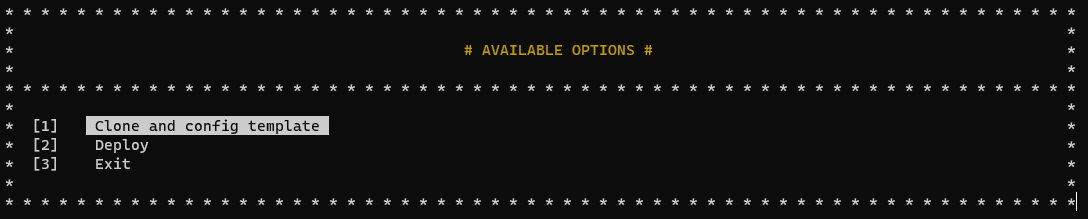
\includegraphics[width=.9\textwidth]{Presentacion/implementacion/script/home.png}
                \caption{Pantalla inicial script}
            \end{figure}            
        \end{center}
        
        
    \end{frame}  

    \begin{frame}{Implementación - Script}
    
        \begin{block}{Clonar plantilla}
            El primer paso para trabajar con el sistema es clonar la plantilla, en caso de ya estarlo se debe eliminar y volver a clonar.          
        \end{block}

        \begin{center}  
            \begin{figure}
                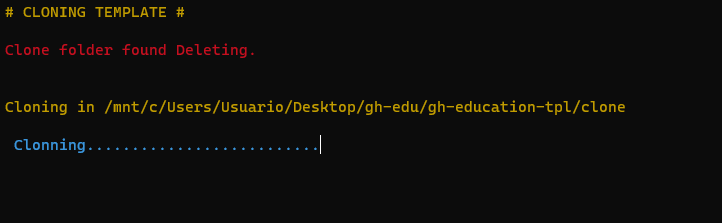
\includegraphics[width=.9\textwidth]{Presentacion/implementacion/script/clone.png}
                \caption{Clonado plantilla}
            \end{figure}            
        \end{center}
        
        
    \end{frame}  

    \begin{frame}{Implementación - Script}
    
        \begin{block}{Autenticación}
            El siguiente paso será autenticarse en Firebase y crear el proyecto de firebase o utilizar uno entre los listados en dicha cuenta.        
        \end{block}

        \begin{center}  
            \begin{figure}
                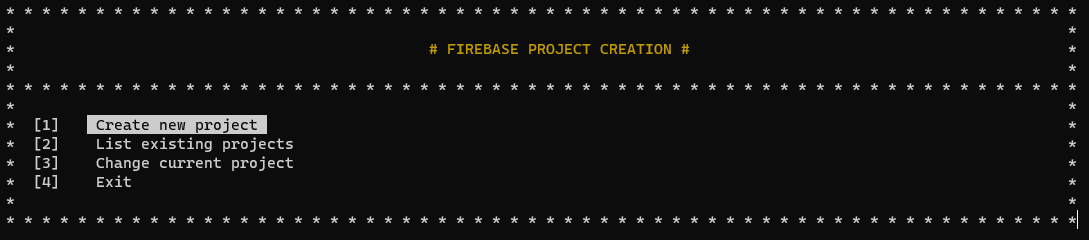
\includegraphics[width=.9\textwidth]{Presentacion/implementacion/script/firebase-initial.png}
                \caption{Menu Firebase}
            \end{figure}            
        \end{center}
        
        
    \end{frame}  

    \begin{frame}{Implementación - Script}

        \begin{center}  
            \begin{figure}
                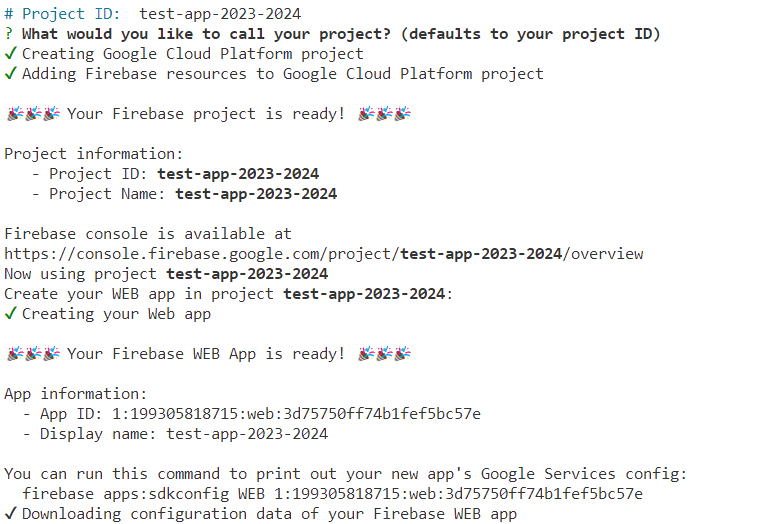
\includegraphics[width=.9\textwidth]{Presentacion/implementacion/script/create-firebase-project.png}
                \caption{Salida creación proyecto Firebase}
            \end{figure}            
        \end{center}
        
        
    \end{frame} 

    \begin{frame}{Implementación - Script}

        \begin{center}  
            \begin{figure}
                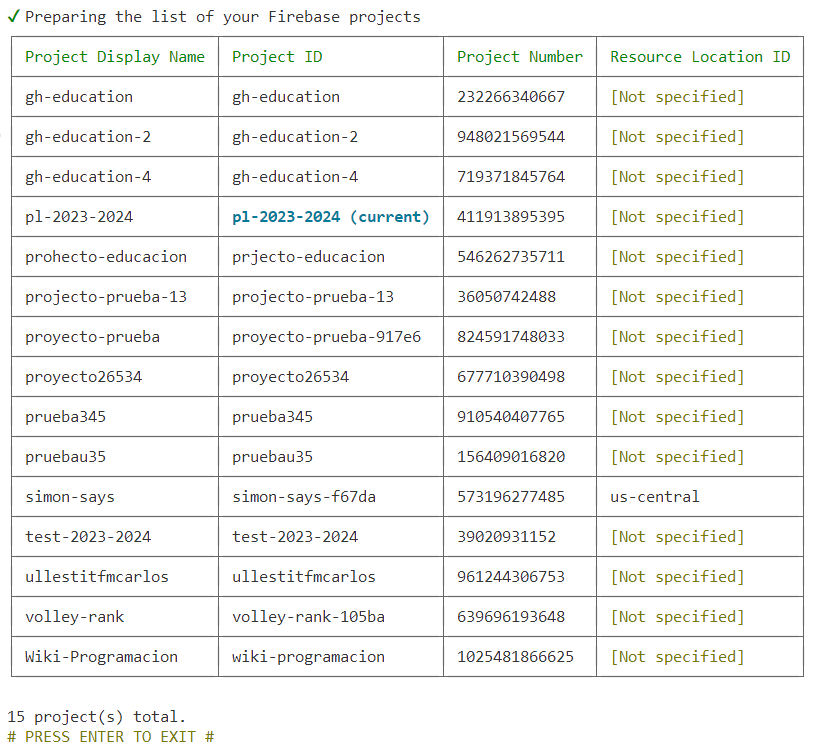
\includegraphics[width=.7\textwidth]{Presentacion/implementacion/script/firebase-list.png}
                \caption{Listado proyectos Firebase}
            \end{figure}            
        \end{center}
        
        
    \end{frame}  

    \begin{frame}{Implementación - Script}
    
        \begin{block}{Despliegue}
            Con Firebase configurado, el siguiente paso es realizar el despliegue. Para facilitar dicha tarea, hay un script que despliega el proyecto apoyándose de un fichero de entorno con variables de configuración. 
        \end{block}

        \begin{center}  
            \begin{figure}
                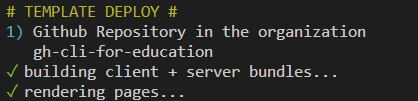
\includegraphics[width=.7\textwidth]{Presentacion/implementacion/script/deploy.png}
                \caption{Despliegue GitHub Pages}
            \end{figure}            
        \end{center}
        
        
    \end{frame}  

    \begin{frame}{Implementación - Plantila}
    
        \begin{block}{Plantilla}
            Para comprender el funcionamiento de la plantilla, se va a hacer un recorrido a través del despliegue que se encuentra en funcionamiento en GitHub.
        \end{block}        

        \href{https://gh-cli-for-education.github.io/gh-education/}{Enlace despliegue en GitHub Pages}
        
    \end{frame}

    \begin{frame}{Conclusiones y Líneas futuras}
        \begin{itemize}
            \item Mejoras de rendimiento en el sistema
            \item Integrar API del LMS (Moodle, Google Classroom,...)
            \item Contemplar casuisticas más complejas
            \item Crear servidores privados para alojar información (no depender de Firebase)
            \item Facilitar personalización desde la web
        \end{itemize}
    \end{frame}  

    \begin{frame}{Bibliografía}

        \bibliographystyle{acm}
        \bibliography{main}
        \nocite{*}
        
    \end{frame}  

\end{document}